\subsection{Working Principle of a 3D Detector}
\begin{frame}
	\frametitle{Working Principle of a 3D Detector}
	\begin{itemize}
		\setlength{\itemsep}{\fill}
		\item insert electrodes perpendicular to the plane
		\begin{itemize}
			\item reduce drift distance
			\item increase collected charge in detectors with limited mean free path %(e.g. irradiated devices)
		\end{itemize}
		\item one readout electrode surrounded by four bias electrodes
		
	\end{itemize}
	\begin{figure}
	  \centering
	  \begin{subfigure}[t]{0.45\textwidth}
		\centering
		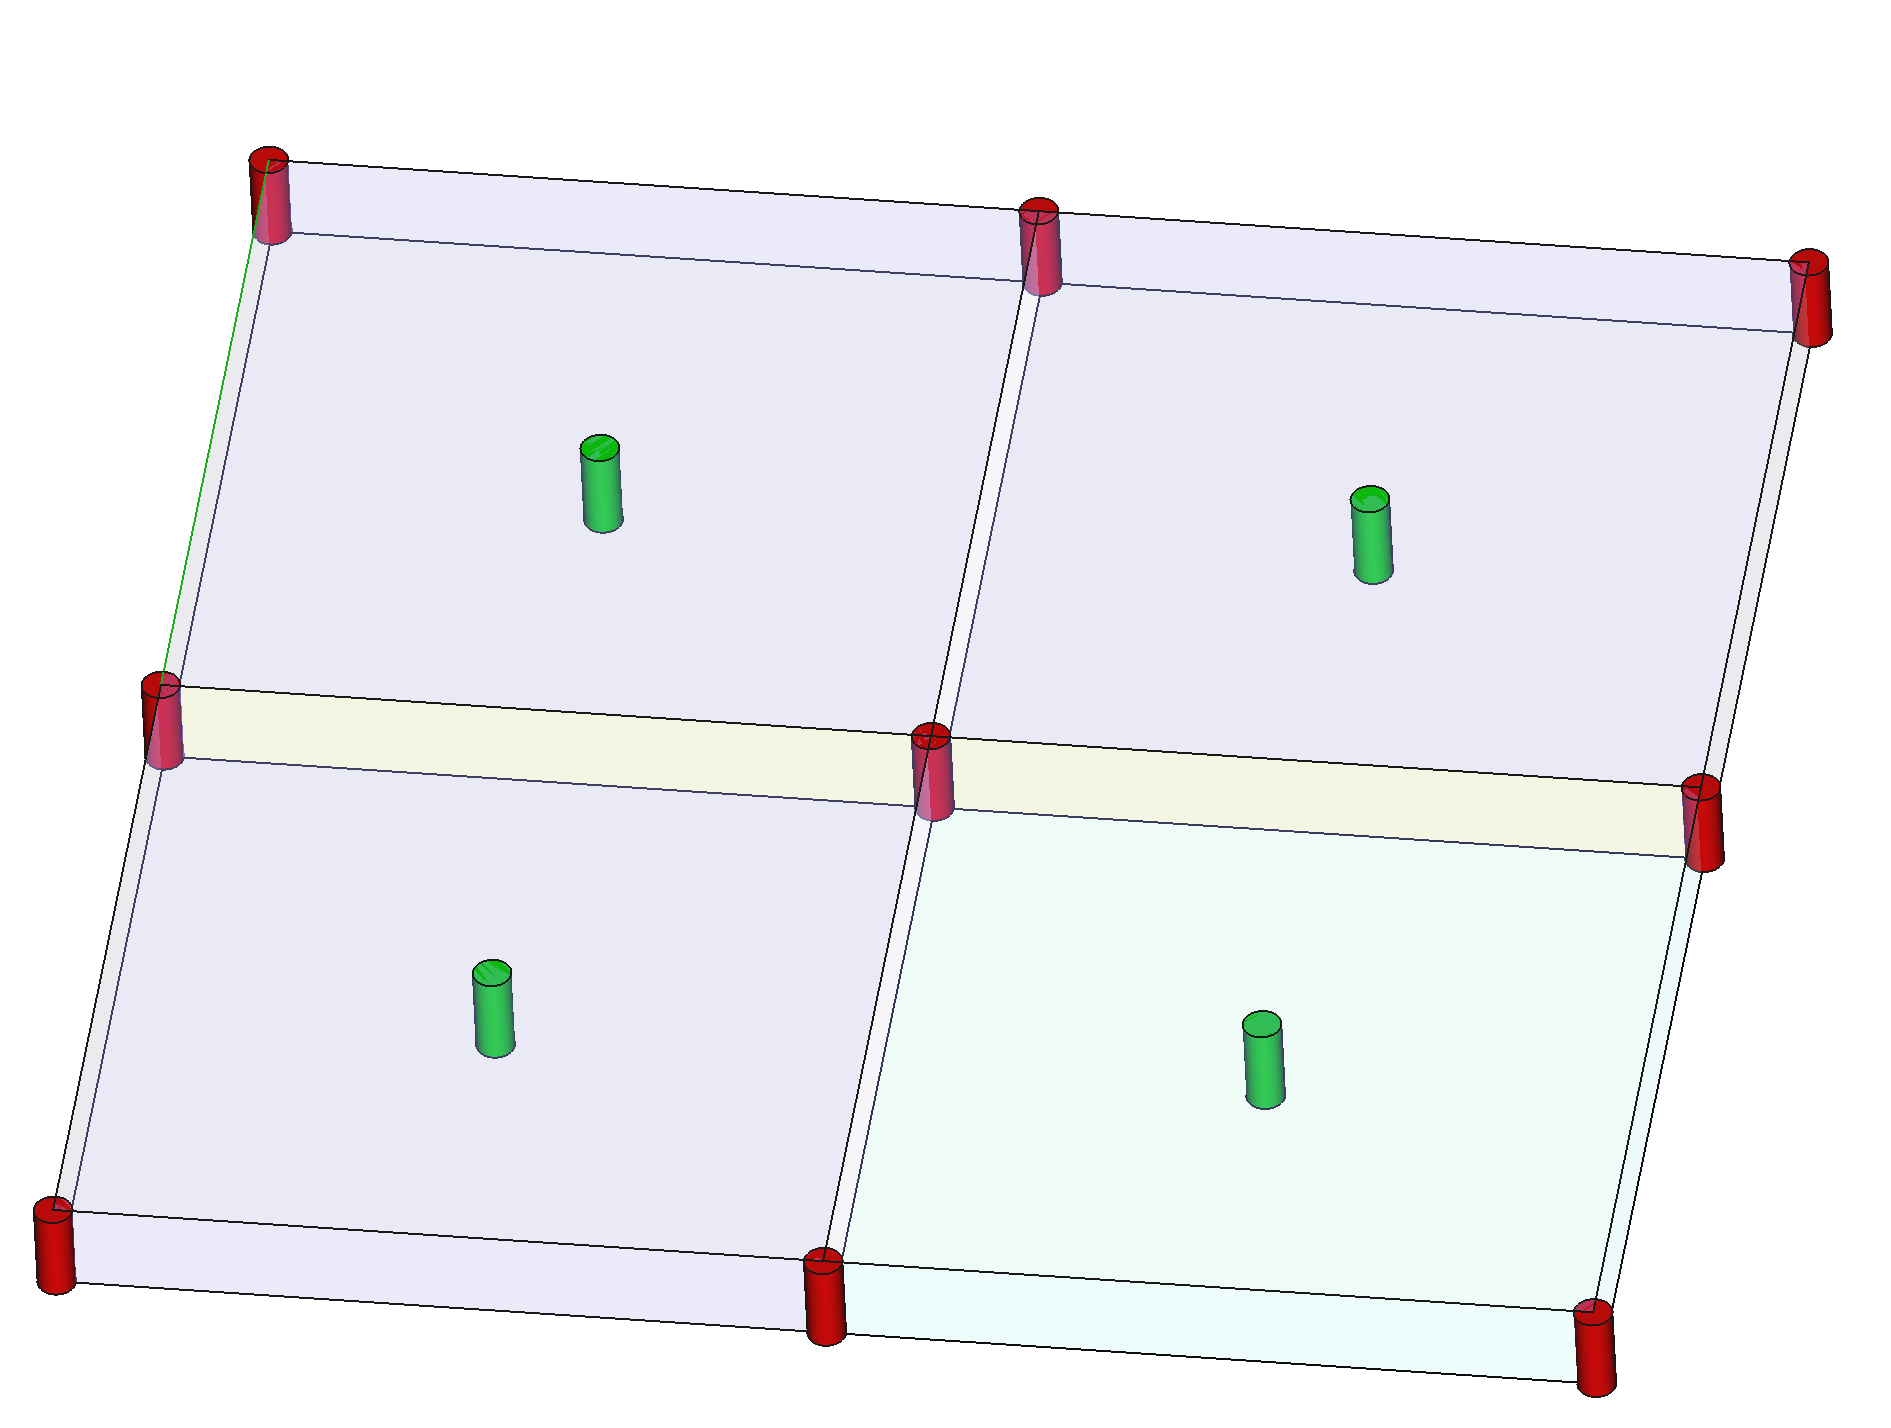
\includegraphics[height=0.4\textheight]{3DScheme}
		\caption{array of four 3D cells, bias electrodes in red, readout electrodes in green}
	  \end{subfigure}
	  \begin{subfigure}[t]{0.45\textwidth}
		\centering
		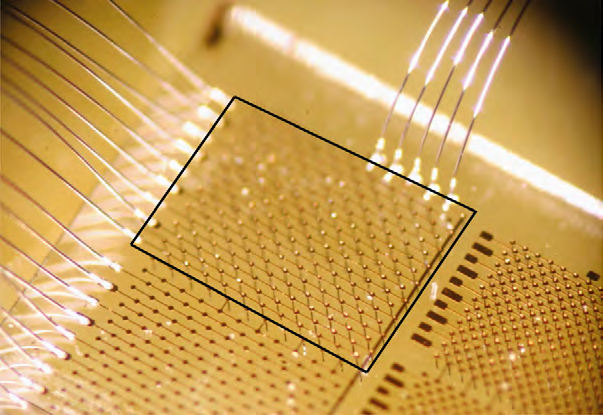
\includegraphics[height=0.4\textheight]{3D}
		\caption{3D diamond detector}
	  \end{subfigure}
	\end{figure}
\end{frame}

% ============================ new frame ==========================================>
\subsection{3D Diamond Detector}
\begin{frame}
	\frametitle{3D Diamond Detector}
	\begin{itemize}
		\item electrodes formed with a pulsed femto second laser (100 fs pulse; 800 nm wavelength)
		\begin{itemize}
			\item transition of diamond to conducting material (graphitic material i.a.)
		\end{itemize}
		\item tested different geometries (4 or 6 bias columns)
    \end{itemize}
	\begin{figure}
		\centering
		\begin{subfigure}[t]{0.45\textwidth}
			\centering
			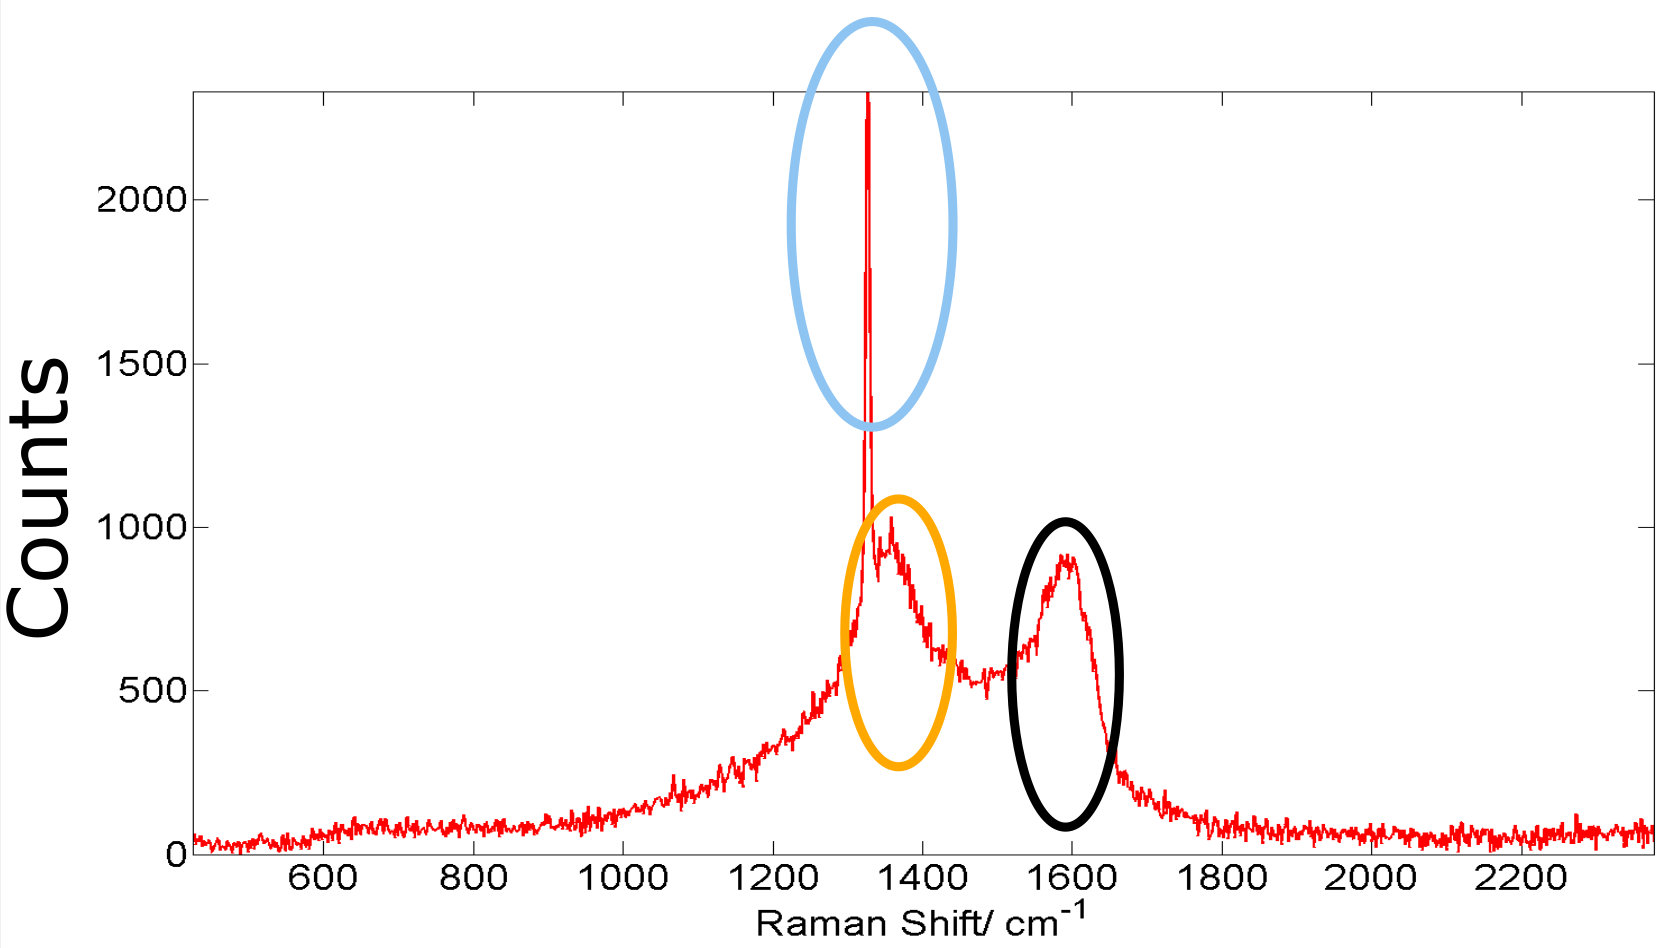
\includegraphics[width=5cm]{raman}
			\caption{blue: Diamond peak. Orange and black: Graphitic material}
		\end{subfigure}
		\begin{subfigure}[t]{0.45\textwidth}
			\centering
			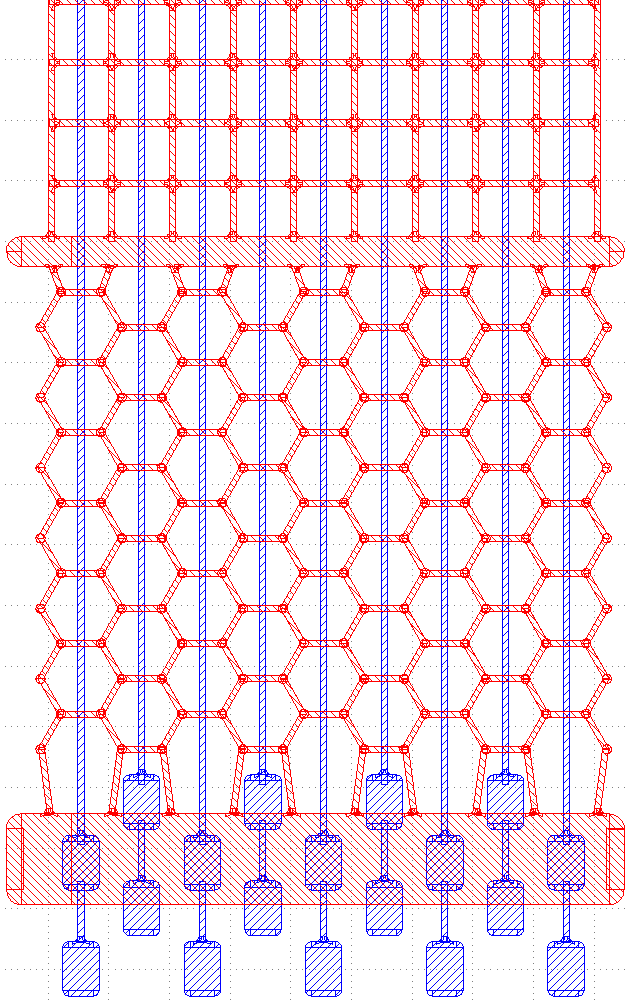
\includegraphics[height=5cm,angle=90]{patterns}
			\caption{square and hexagonal bias patterns (red) and readout channels (blue).}
		\end{subfigure}
	\end{figure}
\end{frame}

% ============================ new frame ==========================================>
\subsection{Beam Tests at CERN}
\begin{frame}
	\frametitle{Beam Tests at CERN}
	\begin{itemize}
		\setlength{\itemsep}{\fill}
		\item using more than 20 years old fixed telescope at SPS at CERN (high spatial resolution)
		\item testing multiple 3D strip detectors with 120GeV protons
		\item basic working principle has been proven
	\end{itemize}
	\begin{figure}
		\centering
		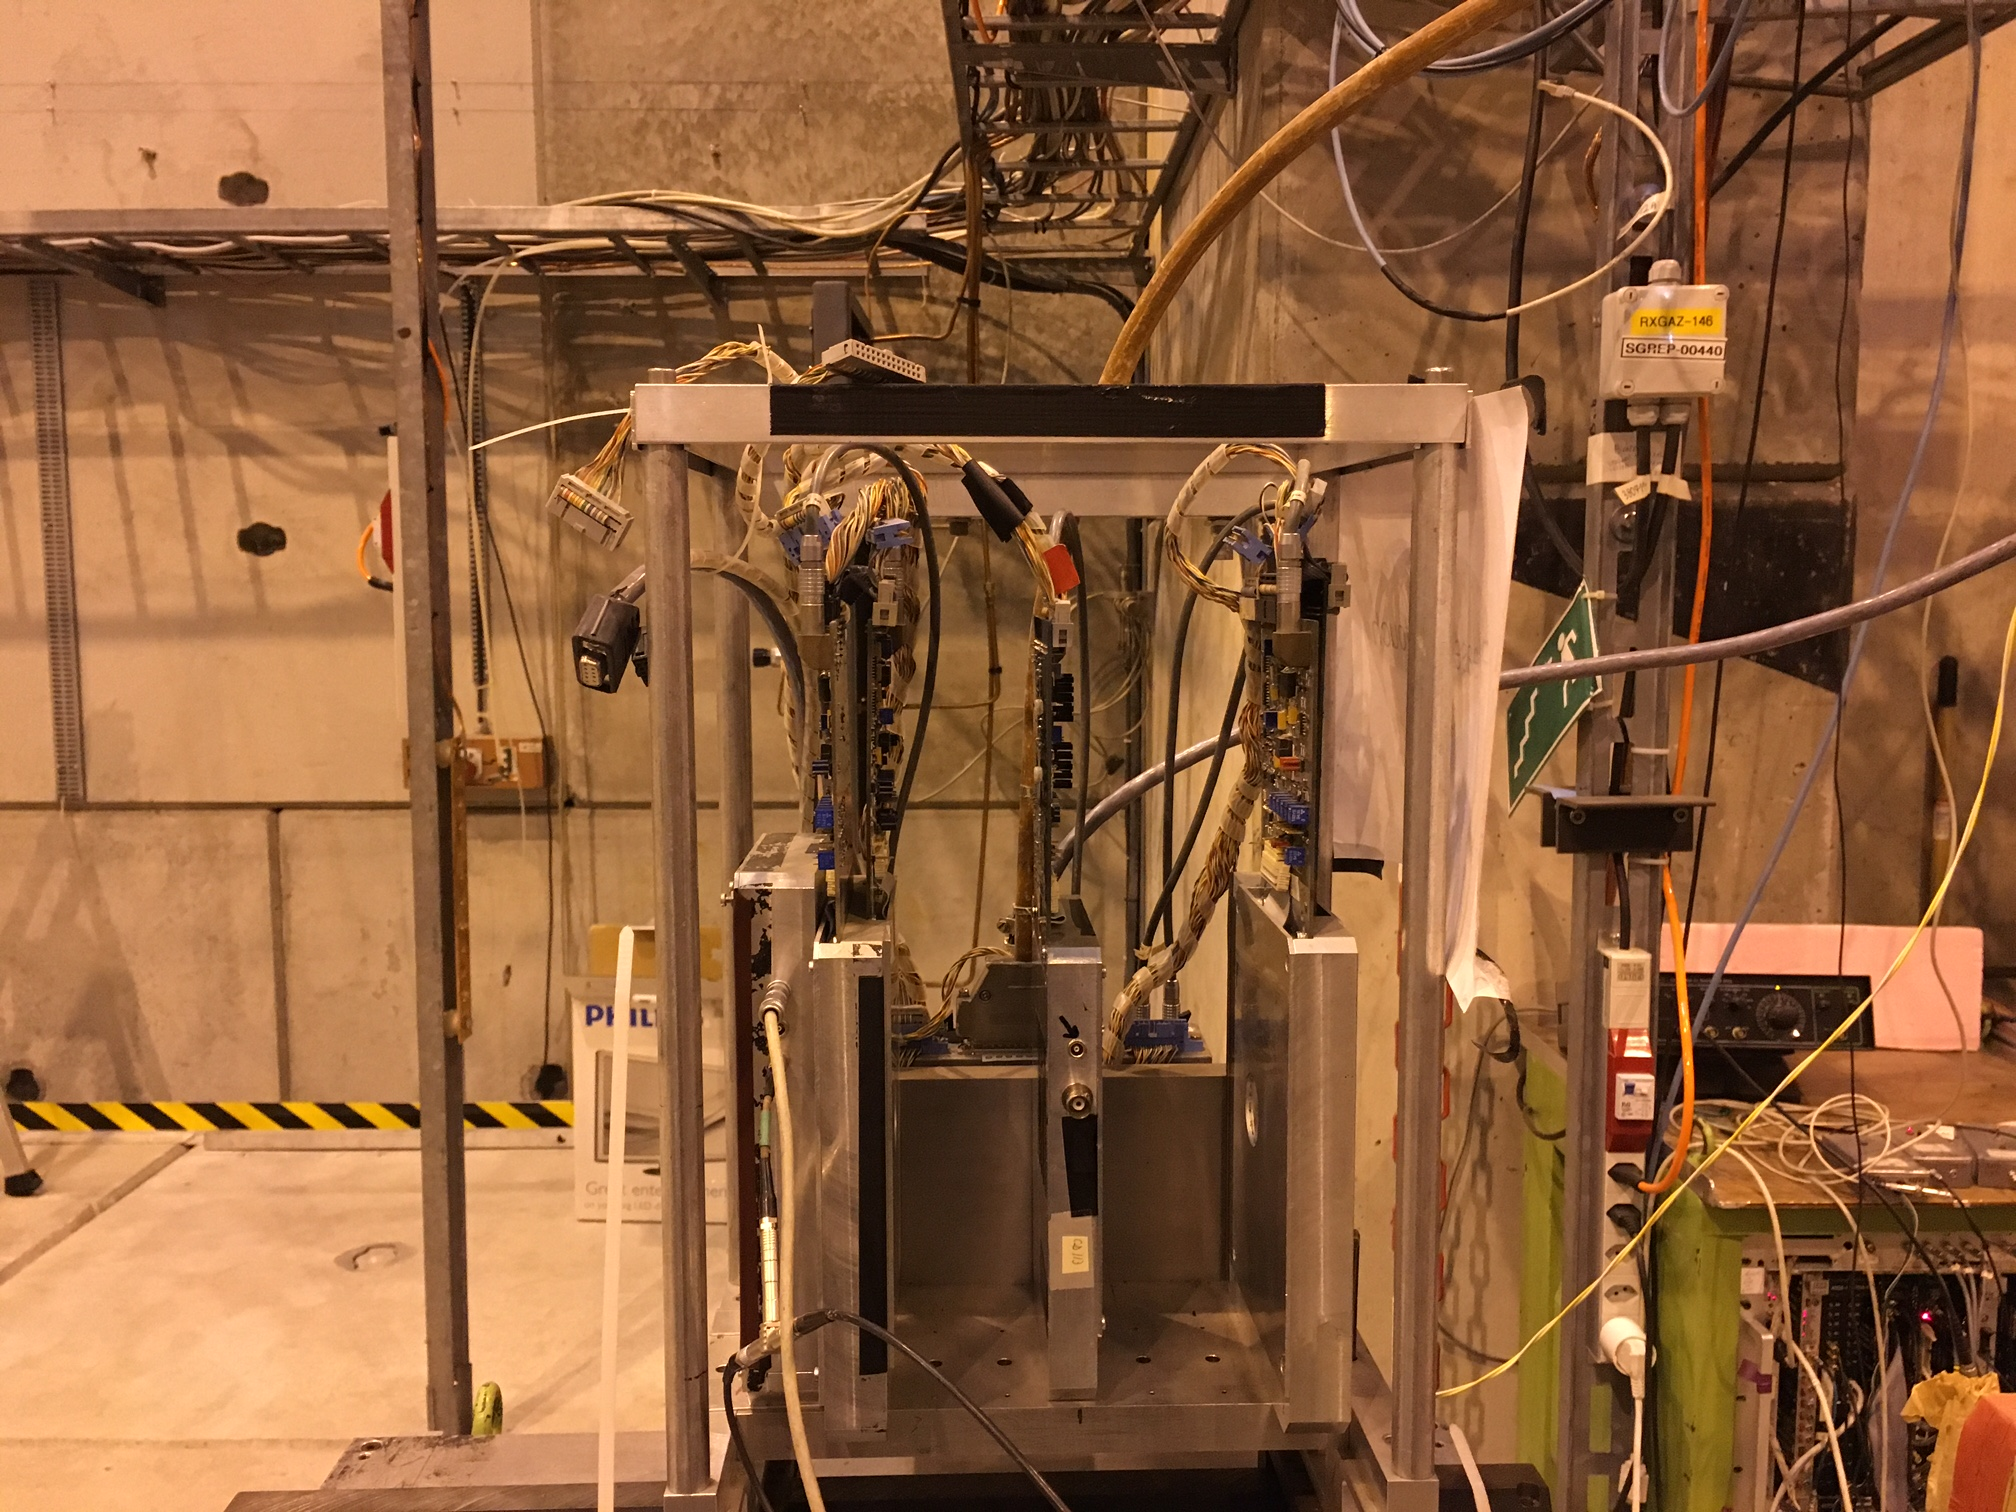
\includegraphics[width=4.5cm]{3DTelescope}
		\caption{Strassbourg Telescope}
	\end{figure}
\end{frame}
% ============================ new frame ==========================================>
\subsection{Analysis}
\begin{frame}
  \frametitle{3D Full detector}
  \begin{itemize}
	\setlength{\itemsep}{\fill}
    \item more than 2000 laser fabricated columns (1152 square cells)    
    \item columns yield \SI{>90}{\%}
    \item \SI{>85}{\%} charge collection for a corresponding thickness
  \end{itemize}
  \begin{figure}[c]
    \centering
    \begin{subfigure}[t]{0.3\textwidth}
      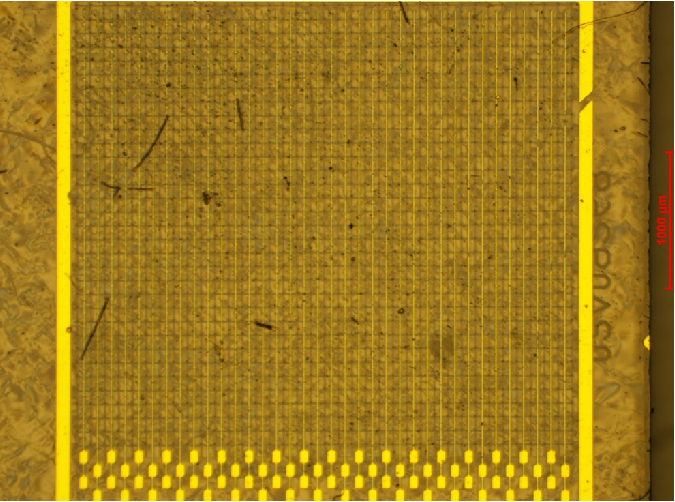
\includegraphics[height=.3\textheight]{large_3D_front}
      \caption{photograph of the metalization pattern in the 3D Full detector}
      \label{fig:3DMetal}
    \end{subfigure}
    \begin{subfigure}[t]{0.3\textwidth}
      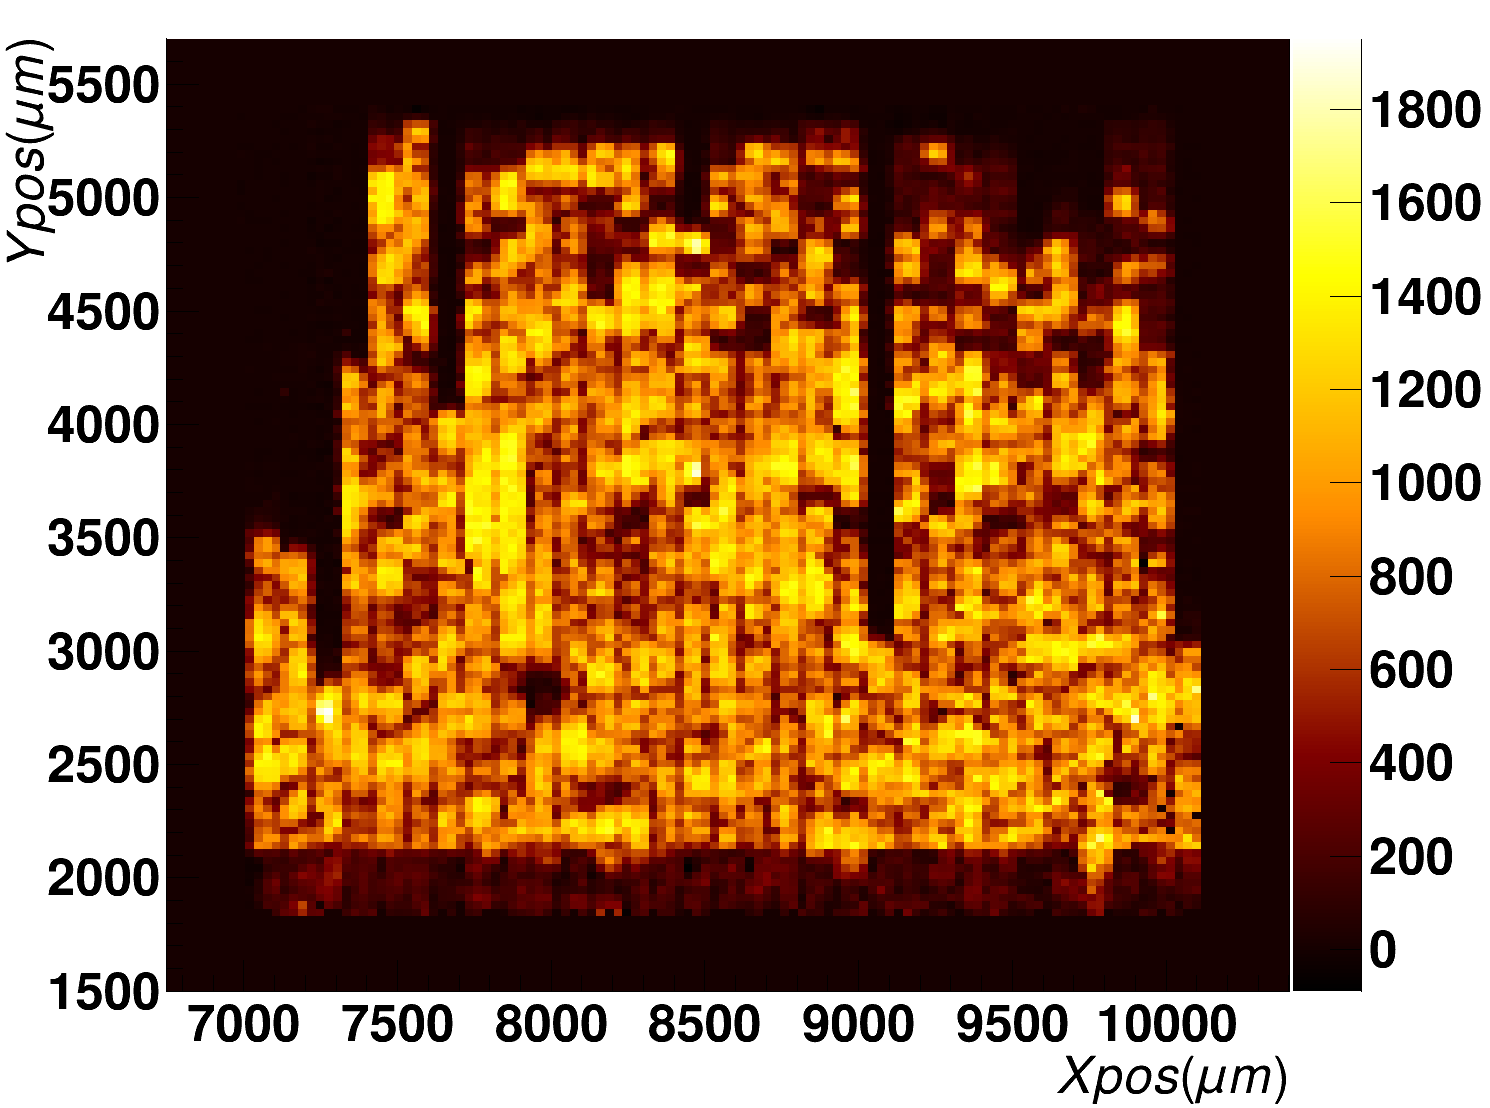
\includegraphics[height=.3\textheight]{SignalMapFull3D}
      \caption{signal map of the 3D Full detector. Broken channels due to fabrication mishandling}
      \label{fig:3dSignalMap}
    \end{subfigure}
    \begin{subfigure}[t]{0.3\textwidth}
      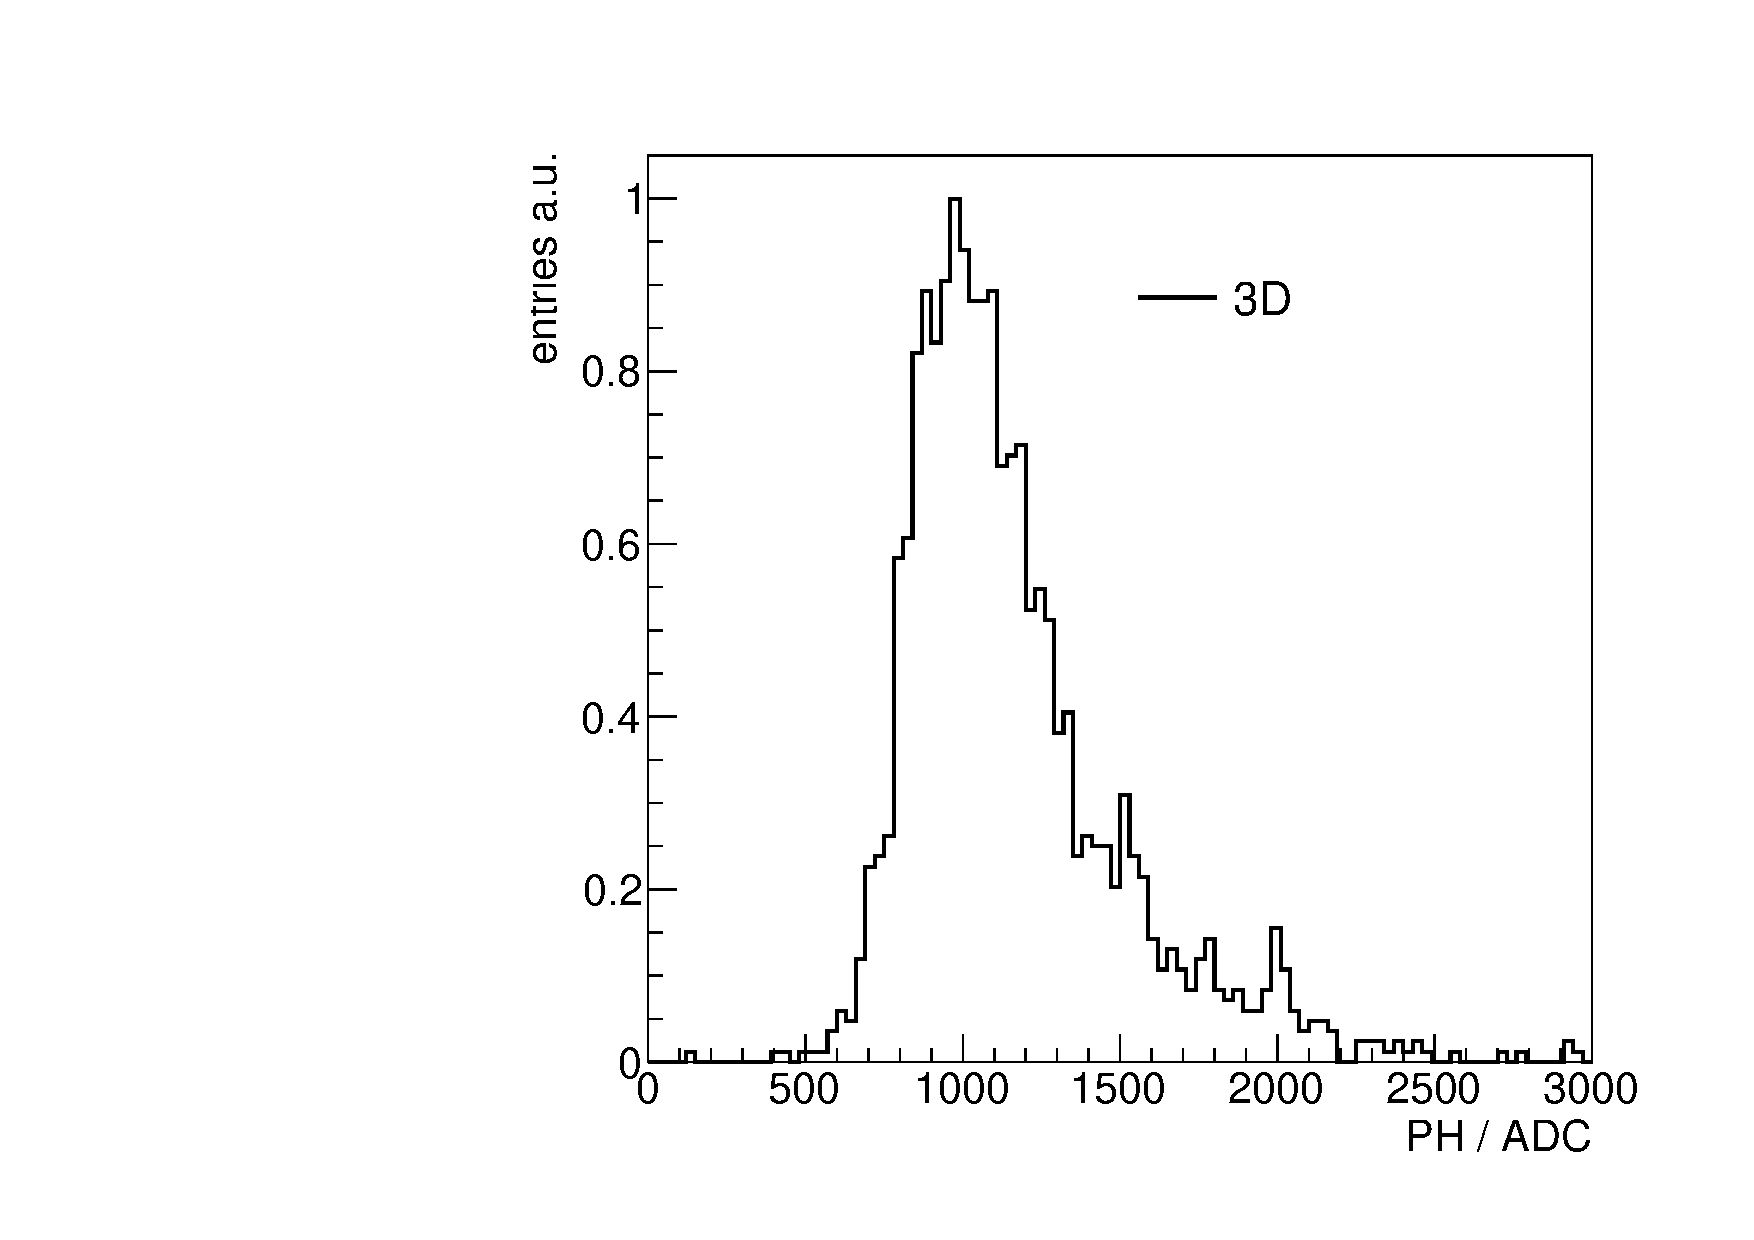
\includegraphics[height=.3\textheight]{large_3D_good_cells_ph}
      \caption{signal distribution of good regions}
      \label{fig:3dhisto}
    \end{subfigure}
  \end{figure}
\end{frame}
% ============================ new frame ==========================================>


